\documentclass[english,version-2022-01]{uzl-thesis} %version-2020-11

\UzLThesisSetup{
  Logo-Dateiname        = {Logo_IMI_de.png},
  Verfasst              = {am}{Institut für Medizinische Informatik},
  Titel auf Deutsch     = {MRT-Registration}, 
  Titel auf Englisch    = {MRT-Registration},
  Autor                 = {Jan Meyer},
  Betreuerin            = {Prof. Dr. Mattias Heinrich},
  Mit Unterstützung von = {Ziad Al-Haj Hemidi, Eytan Kats},
  Masterarbeit,
  Studiengang           = {Medizinische Informatik},
  Datum                 = {1. Januar 2025},
  Abstract              = {Something about MRI and registration},
  Zusammenfassung       = {Irgendwas über MRT und Registration},
  Acknowledgements      = {Danke an Mattias, Ziad und Eytan für die gute Betreuung.},
  Numerische Bibliographie %Alphabetische
}


% Designs
%\UzLStyle{computer modern oldschool design}
%\UzLStyle{computer modern scholary design}
%\UzLStyle{pagella basic design}
%\UzLStyle{pagella centered design}
%\UzLStyle{pagella contrast design}
%\UzLStyle{alegrya basic design}
%\UzLStyle{alegrya scholary design}
%\UzLStyle{alegrya stylish design}
\UzLStyle{alegrya modern design}




%%%%%%%%
%
% Now, include the package you need here using \usepackage. 
%
% However, many standard packages are already loaded by the class:
% amsmath, amssymb, amsthm, babel, biblatex, csquotes, etoolbox,
% filecontents, fontspec, geometry, hyperref, tikz (with libraries
% arrows.meta, positioning and shapes), varioref, url 
%
%%%%%%%
\usepackage{subcaption}


% add bibliography
%\addbibresource{Bibliography.bib}
\bibliography{Bibliography.bib}


\begin{document}

%%%%%%%%%%%%%%%%%%%%%%%%%
%%%%%  Introduction %%%%%
%%%%%%%%%%%%%%%%%%%%%%%%%

\chapter{Introduction}
Introduction of stuff.

\section{Contributions of the Thesis}
We implemented stuff.

\section{Related Work}
There are many papers on image registration in general, however in the context of medical image registration with deep learning their number is reduced due to the specialized nature of the subject at hand. Yet, there are a couple of papers that give a good overview of the topic.
They give a brief overview of registration methods, basics of deep learning with already existing networks for image registration as well as covering potential applications and challenges~\cite{Chen2020,Haskins2020,Fu2020,Zou2022,Chen2023}.
A lot of different approaches for medical image registration are based on \emph{VoxelMorph}~\cite{Voxelmorph}, such as both \emph{Fourier-Net}~\cite{Fourier-Net} and its successor \emph{Fourier-Net+}~\cite{Fourier-Net+}.


\section{Structure of the Thesis}
This Thesis contains a lot of stuff in different chapters.

%%%%%%%%%%%%%%%%%%%%%%%
%%%%%%%  Basics %%%%%%%
%%%%%%%%%%%%%%%%%%%%%%%

\chapter{Basics}
In this chapter the basics of the thesis are explained.

\section{Magnetic Particle Imaging}
Here MRI is described. % TODO: define abbreviations for CT and MRI here!!

\section{Image Registration}
Image registration is a challenging, yet important task for image processing. It can be described as the process of transforming different
image datasets into one coordinate system with matched imaging contents~\cite{Haskins2020}. In the medical field this can be used for clinical applications such as disease diagnosis and monitoring, image-guided treatment delivery, and post-operative assessment. Medical image registration is typically used to preprocess data for tasks like object detection (for e.g. tumor growth monitoring) and segmentation (for e.g. organ atlas creation) where variation in spatial resolution is common between modalities like CT and MRI and patients. Thus the performance of these methods is dependent on the quality of image registration~\cite{Chen2020}. \\
Medical image registration was often done manually by clinicians, however, registration tasks are often challenging and the quality of manual alignments is dependent on the expertise of the user. These manual registrations are thus not only time consuming, but also hardly reproducible leading to high interobserver-variability. The need for automatic registration is very much apparent, but this task remained hard to solve for a long time, requiring a lot of computational power and time for computer algorithms to solve the problem. While neural networks also require a lot of computational power and time to train, they promise fast execution after training. With the rise of deep learning these network gained popularity and now pose a real alternative to conventional algorithms and manual registration~\cite{Haskins2020}. We will discuss these new approaches in the next section, but first we need to formally define our problem.\\
In pair-wise image registration two images ($F$ and $M$) are to be aligned, with $F$ denoting the fixed and $M$ the moving image. T is the desired spatial transformation that aligns the two images. This can be posed as an optimization problem:
\begin{equation}
	T' = \arg\max S(F, T(M)),
\end{equation}
with $T'$ being the best transformation that maximizes the similarity $S$ between the two images. This process is done iteratively improving estimates for the desired T, such that the defined similarity in the cost function is maximized~\cite{Chen2020}.\\
Transformations can be categorized as rigid, affine, and deformable. A rigid transformation consists of rotation and translation; an affine transformation
includes translations, rotations, scaling, and sheering; the two kinds of transformations are described as a 2D single matrix. Unlike rigid and affine transformation, deformable transformation is a high-dimension problem that we need to formulate by a 3D matrix for 2D deformable registration i.e., a so-called deformation field. While rigid and affine registration algorithms have already achieved good performance in many applications, deformable registration is still a challenging task due to its intrinsic complexity, particularly when the deformation is large. However, these are also the transformations most likely encountered in clinical practice as it can be utilized to fuse information from different modalities such as MRI and CT~\cite{Zou2022}. Additionally, deformable image registration can also be
utilized for various computer-assisted interventions like biopsy~\cite{Tam2016} and (MRI-guided) radiotherapy~\cite{Chen2017, Rigaud2019}. \\
Intuitively, deformable image registration is an ill-posed problem, making it fundamentally different from other computer vision tasks such as object localization, segmentation or classification. Given two images, deformable image registration aims to find a spatial transformation that warps the moving image to match the fixed image as closely as possible. However, there is no ground-truth available for the desired deformation field and without enforcing any constraints on the properties of the spatial transformation, the resulting cost function is ill-conditioned and highly non-convex. In order to address the latter and ensure tractability, all image registration algorithms regularize the estimated deformation field, based on some prior assumptions on the properties of the underlying unknown deformation~\cite{Chen2020}.\\
Many methods have been proposed for medical image registration to deal with the complex challenges of this task. Popular conventional registration methods include optical flow~\cite{Yang2008}, demons~\cite{Vercauteren2009} and many more. However, most of these still lack accuracy and computation speed, which makes newer deep learning approaches all the more interesting~\cite{Fu2020}.

\section{Deep Learning Architectures}
Neural networks, despite the theoretical concepts being around for decades, have seen a meteoric rise in popularity over the last few years as constraints on computational power have been alleviated. Especially deep neural networks, which are often summarized under the term deep learning (DL). Recent years have witnessed an almost exponential growth in the development and use of DL algorithms, sustained thus far by rapid improvements in computational hardware (e.g. GPUs). Consequently, clinical applications requiring image classification, segmentation, registration, or object detection/localization, have witnessed significant improvements in algorithmic performance, in terms of accuracy and/or efficiency~\cite{Chen2020}. The following network architecture are widely used for different tasks including medical image registration. \\
Some basic stuff about network training, testing and different architectures that are relevant for the later Chapters.

\subsection{Convolutional Neural Networks}
Convolutional neural networks (CNNs) are a type of deep neural networks with regularized multilayer perceptron, which are mainly used for image processing. CNNs use convolution operations instead of general matrix multiplications in typical neural networks. These convolutional filters make CNNs very suitable for visual signal processing. Because of their excellent feature extraction ability, CNNs are some of the most successful models for image analysis. Different variants of CNN have been proposed and have achieved the-state-of-art performances in various image processing tasks. A typical CNN usually consists of multiple convolutional layers, max pooling layers, batch normalization layers, sometimes dropout layers, a sigmoid or softmax layer. In each convolutional layer, multiple channels of feature maps are extracted by sliding trainable convolutional kernels across the input feature maps. Hierarchical features with high-level abstraction are extracted using multiple convolutional layers. These feature maps usually go through multiple fully connected layer before reaching the final decision layer. Max pooling layers are often used to reduce the image sizes and to promote spatial invariance of the network. Batch normalization is used to reduce internal covariate shift among the training samples. Weight regularization and dropout layers are used to alleviate data overfitting~\cite{Fu2020}. The loss function is often defined as the difference between the predicted and the target output. CNNs are usually trained by minimizing the loss via gradient back propagation using optimization methods like Adam~\cite{Adam}. 

\subsection{U-Net}
The U-Net~\cite{U-Net} architecture is an extension of the typical CNNs structure typically used for image segmentation, however it can also be used for image registration tasks. It adopts symmetrical contractive and expansive paths with skip connections between them. The encoding blocks on the left extract important features from the image using convolution layers and max pooling, which are then stored in the latent space in the middle. From there it is reconstructed using upsampling and convolutions in the decoding blocks on the right. Additionally, skip connections are used to improve the spatial resolution of the segmentation. This architecture allows effective feature learning from a small number of training datasets~\cite{Fu2020}. 

\subsection{Autoencoders}
An autoencoder (AE) is a type of CNNs that learns to reconstruct an image from its input without supervision. AEs usually consists of an encoder which extracts the input features, which are stored a low-dimensional latent state space, similar to a U-Net, and a decoder which restore the original input from the latent space. To prevent an AE from learning an identity function, regularized autoencoders were invented, which can be used for e.g. denoising AEs. Variational AEs (VAEs) are generative models that learn latent representation using a variational approach, which constrains the variability of the outputs. VAEs can been used for anomaly detection and image generation~\cite{Fu2020}.

\subsection{Generative Adversarial Networks}
Generative adversarial networks (GANs) consist of two competing networks, a generator and a discriminator. The generator is trained to generate artificial data that approximate a target data distribution from a low-dimensional latent space similar to an AE. The discriminator is trained to distinguish the artificial data from actual data. The discriminator encourages the generator to predict realistic data by penalizing unrealistic predictions via learning. Therefore, the discriminative loss could be considered as a dynamic network-based loss term. The generator and discriminator both are getting better during training to reach Nash equilibrium. In medical imaging, GANs have been used to perform image synthesis for inter- or intra-modality, such as MRI to synthetic CT and vise versa. In medical image registration, GANs are usually used to either provide additional regularization or translate multi-modal registration to uni-modal registration~\cite{Fu2020}.

\section{Deep Learning for Image Registration}
Recently, there has been a surge in the use of deep learning based approaches for medical image registration. Their success is largely due to their ability to perform fast inference, and the flexibility to leverage auxiliary information such as anatomical masks as part of the training process. The most effective methods, such as \emph{VoxelMorph}~\cite{Voxelmorph}, typically employ a U-Net style architecture to estimate dense spatial deformation fields. These methods require only one forward pass during inference, making them orders of magnitude faster than traditional iterative methods. Following the success of \emph{VoxelMorph}, numerous deep neural networks have been proposed for various registration tasks~\cite{Fourier-Net+}. Other approaches also utilize CNNs, AEs and GANs. Typical strategies are discussed in more detail in the following sections.

\subsection{Supervised Registration}
Supervised registration describes training a network with a ground truth displacement field that is either real (created by hand) or synthetic (generated via traditional iterative registration algorithms). Thus the loss can easily be calculated as the difference in the displacement fields of the network prediction and the ground truth. These methods have achieved notable results with real displacement fields as supervision. However, this approach is very limited by the size and the diversity of the dataset. As the displacement fields are often calculated by conventional algorithms their effectiveness might be limited for difficult problems with which the traditional algorithms struggle. Fully supervised methods are widely studied and have notable results, but the generation of real or synthetic displacement fields is hard, and these displacements fields might be different from the real ground truth, which can impact the accuracy and efficiency of these kinds of methods~\cite{Zou2022}. Notable approaches include \emph{BIRNet}~\cite{BIRNet}.

\subsection{Unsupervised Registration}
As the preparation of the ground truth displacement field for supervised methods is inconvenient, limitations in generalizing results in different domains and various registration tasks are inevitable. Thus, unsupervised registration has a more convenient training process with paired images as inputs, but without a ground truth. Generally, unsupervised learning consists of similarity-based and GAN-based methods, where the loss function computes the similarity between the aligned images and the smoothness of the displacement field, rather than the difference to a ground truth~\cite{Zou2022}. Well known example are \emph{IC-Net}~\cite{IC-Net},  \emph{VoxelMorph}~\cite{Voxelmorph}, \emph{TransMorph}~\cite{TransMorph} and \emph{SYMNet}~\cite{SYM-Net}.


%%%%%%%%%%%%%%%%%%%%%%%%
%%%%%  Methodology %%%%%
%%%%%%%%%%%%%%%%%%%%%%%%

%\chapter{Methodology}
%In this chapter the main part of the actual work is discussed.

\chapter{Data}
Here the datasets are described.

\section{OASIS}
For training and testing the \emph{OASIS-1} dataset~\cite{OASIS} was mainly used, which contains T1-weighted MRI brain scans from 454 subjects. These were further pre-processed by~\cite{HyperMorph} for the \emph{Learn2Reg}-Challenge~\cite{Learn2Reg}. This enables subject-to-subject brain registration, as all MRI scans were bias-corrected, skull-stripped, aligned, and cropped to the size of $160 \times 192 \times 224$. Examples can be seen in Figures~\ref{fig:image1} and \ref{fig:image2} with slices from the center of the x-, y- and z-axis.

\begin{figure}[htpb]
	\centering
	\graphicspath{{images/}{\main/images/}}
	\begin{subfigure}{0.45\textwidth}
    		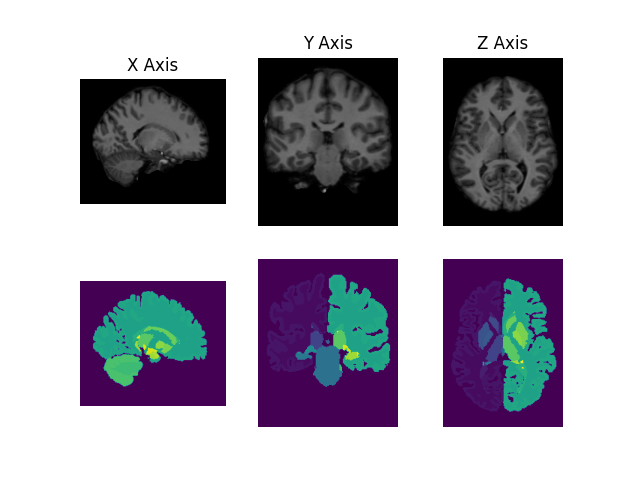
\includegraphics[width=\textwidth]{image2.png}
    		%\caption{Example Image from the Dataset with corresponding labels.}
		\caption{}    		
    		\label{fig:image2}
	\end{subfigure}
	\hfill
	\begin{subfigure}{0.45\textwidth}
    		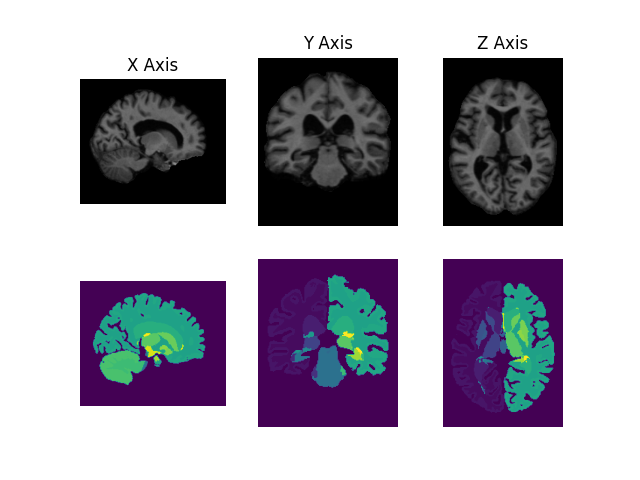
\includegraphics[width=\textwidth]{image1.png}
    		%\caption{Another example Image from the Dataset with corresponding labels.}
		\caption{}    		
    		\label{fig:image1}
	\end{subfigure}
	\caption{Example images (upper row) from the \emph{OASIS} dataset with corresponding labels (bottom row).}
	\label{fig:OASIS}
\end{figure}


\chapter{Network Architectures}
As a starting point \emph{Fourier-Net}~\cite{Fourier-Net} and its successor \emph{Fourier-Net+}~\cite{Fourier-Net+} were used. These networks, which are explained in the following pages, enable fast and accurate registration while needing less resources compared to similar approaches. But we also did our own stuff...

\section{Fourier-Net}
\emph{Fourier-Net} is a new unsupervised approach that aims to learn a low-dimensional representation of the displacement field in a band-limited Fourier domain instead of the full field in the spatial domain. This band-limited representation is then decoded by a model-driven decoder to the dense, full-resolution displacement field in the spatial domain. This allows for fewer parameters and computational operations, resulting in faster inference speeds~\cite{Fourier-Net}. The architecture is based on the U-Net~\cite{U-Net}, like most deep registration approaches, but replaces the expansive path with a parameter-free model-driven decoder as mentioned before. The encoder of \emph{Fourier-Net} consists of a CNN and takes two images (fixed and moving) as inputs. The output is a displacement field that is then converted from the spatial domain into the Fourier domain via an discrete Fourier transformation (DFT) and band-limiting by low-pass filtering. From there, this band-limiting representation 
%of the displacement field 
is padded with zeros to the full resolution of the original displacement field. The field is then recovered by using the inverse DFT (iDFT) to convert it back into the spatial domain. This displacement field is then used to warp the moving image into the fixed image. Additionally, squaring and scaling layers~\cite{Dalca2018} can be added before warping the image in order to encourage a diffeomorphism in final deformation. 

\begin{figure}[htpb]
	\centering
	\graphicspath{{images/}{\main/images/}}
	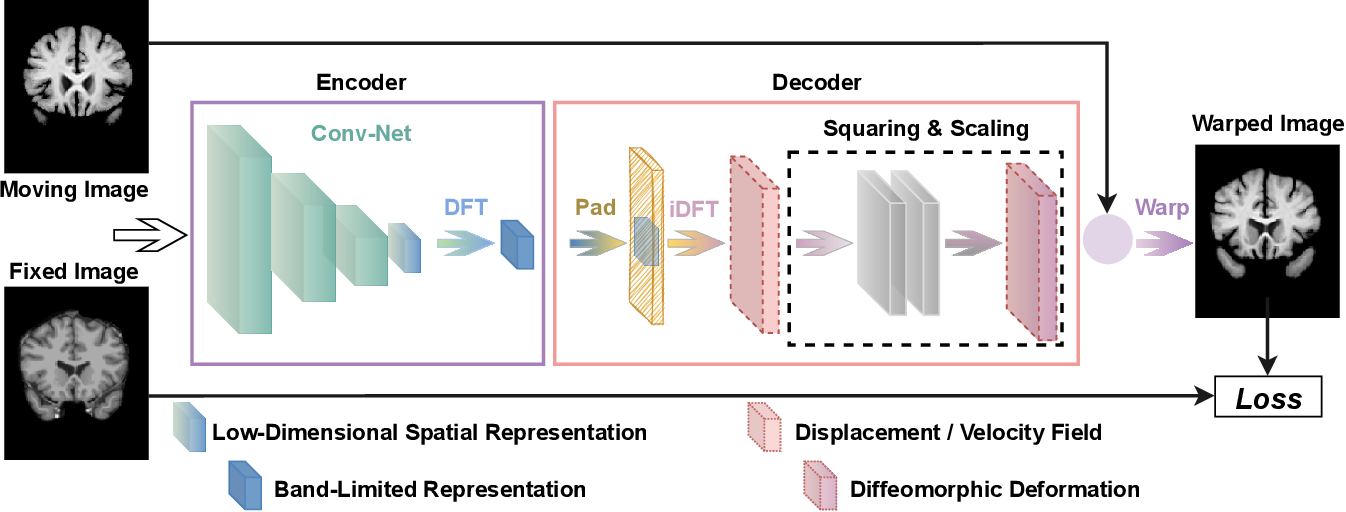
\includegraphics[width=\linewidth]{ArchitectureFourier-Net.png} 
	\caption{Architecture of \emph{Fourier-Net} taken from~\cite{Fourier-Net}.}
	\label{fig:Fourier-Net}
\end{figure}

\subsection{Encoder}
Describe SYMNet, etc. in more detail here.\\
The encoder of \emph{Fourier-Net} consists of a CNN, namely the \emph{SYMNet}~\cite{SYM-Net}.

\subsection{Decoder}
Describe DFT, etc. here.

\subsection{Diffeomorphism}
Describe what a diffeomorphism is. Describe Squaring and Scaling layers.\\
A diffeomorphic deformation is defined as a smooth and invertible deformation, thus the output of the iDFT layer can be regarded as a stationary velocity field denoted by $v$ instead of the displacement field $\theta$. In group theory, $v$ is a member of Lie algebra, and it can be exponentiated to obtain the diffeomorphic deformation. This specific version is then called \emph{Fourier-Net Diff} A diagram of this can be seen in Figure~\ref{fig:Fourier-Net}. 

\subsection{SpatialTransformer}
Describe the Spatial Transformer.\\
For this warping layer the \emph{spatial transformer}~\cite{SpatialTransformer}
%similar to~\cite{Voxelmorph} 
is used.

\subsection{Loss Function}
Describe Parts of the loss function.\\After the moving image has been warped the unsupervised loss $\mathcal{L}$ can be calculated as follows:
\begin{equation}
	\mathcal{L}(\Theta) = \min \bigg[ \bigg( \frac{1}{N} \sum^{N}_{i=1} \mathcal{L}_{Sim} (I_{M_i} \circ (\phi_i(\Theta) + \text{Id}) - I_{F_i}) \bigg) + \lambda \cdot \bigg( \frac{1}{N} \sum^{N}_{i=1} || \nabla \phi_i(\Theta) ||^2_2 \bigg) \bigg] ,
\end{equation}
where $\circ$ denotes the warping operation, $N$ the number of training pairs with moving images $I_{M_i}$ and fixed images $I_{F_i}$, $\Theta$ the network parameters, $\phi$ the displacement field, Id the identity grid and $\nabla$ the first order gradient. The two terms of the loss, $\mathcal{L}_{Sim}$ determining the similarity between warped moving images and fixed images via MSE or NCC, and the second term defining the smoothness of the displacement fields, are balanced using the scalar parameter $\lambda$.\\
When using the squaring and scaling layers, thus making the deformation of the moving image diffeomorphic, the loss can be modified by replacing the displacement field $\theta$ with the velocity field $v$:
\begin{equation}
	\mathcal{L}(\Theta) = \min \bigg[ \bigg( \frac{1}{N} \sum^{N}_{i=1} \mathcal{L}_{Sim} (I_{M_i} \circ Exp(v_i(\Theta) - I_{F_i}) \bigg) + \lambda \cdot \bigg( \frac{1}{N} \sum^{N}_{i=1} || \nabla v_i(\Theta) ||^2_2 \bigg) \bigg] .
\end{equation}

\subsection{Training}
Describe how to reproduce results from the paper...\\
\emph{Fourier-Net} can be used with both 2D as well as 3D inputs, however the latter are harder to visualize. As the \emph{OASIS} dataset provides 3D volumes with annotations we can slice these to get 2D image data with matching labels (see Figure~\ref{fig:OASIS} for the calculation of the Dice-Score. Thus we can nicely visualize the training success of the 2D network by locking at the difference between images before and after registration in addition to the Dice-Score, which can also be calculated for 3D data.  This can be seen in Figure~\ref{fig:DifferencesTrainingProgress} with two examples from different stages of the training process. Despite the example in Figure~\ref{fig:Training29600it} being the far harder example to align the network performs better than before (see Figure~\ref{fig:Training800it}) due to the training progress.

\begin{figure}[htpb]
	\centering
	\graphicspath{{images/}{\main/images/}}
	\begin{subfigure}{0.45\textwidth}
		\centering
    		\includegraphics[width=\textwidth]{results1.png}
    		\caption{Training progress after 800 iterations.}
    		\label{fig:Training800it}
	\end{subfigure}
	\hfill
	\begin{subfigure}{0.45\textwidth}
		\centering
    		\includegraphics[width=\textwidth]{results2.png}
    		\caption{Training progress after 29600 iterations.}
    		\label{fig:Training29600it}
	\end{subfigure}
	\caption{Differences between moving and fixed images before and after registration.}
	\label{fig:DifferencesTrainingProgress}
\end{figure}


\section{Fourier Net+}
\emph{Fourier-Net+}, as the name suggests, is an extension of Fourier-Net which takes the band-limited spatial representation of the images as input, instead of their original full-resolution counterparts. This leads to further reduction in the number of convolutional layers in the contracting path of the network, resulting in a decrease of parameters, memory usage, and computational operations. This makes \emph{Fourier-Net+} even more efficient than its older predecessor~\cite{Fourier-Net+}.\\
As seen in Figure~\ref{fig:Fourier-Net+}, the network architecture is almost the same as for \emph{Fourier-Net} (see Figure~\ref{fig:Fourier-Net} for reference). However, while the decoder, and thus the loss function, remain the same, the encoder is slightly altered to make the network even more efficient. For this, similarly to the decoder, a DFT is used, however this time the idea is applied to the input images. These are first transformed into the Fourier domain, then low-pass filtered and finally reconstructed from their band-limited representation back into the spatial domain via an iDFT. The two images, now compressed, are the input for the encoder of \emph{Fourier-Net}, meaning the CNN and following DFT. However, due to the band-limiting before the CNN, the latter can be made much more light-weight, thus reducing computational cost. This is visualized in Figure~\ref{fig:Fourier-Net+CNN}. Thus, \emph{Fourier-Net+} too is overall lighter than the baseline \emph{Fourier-Net} in terms of the number of parameters and computations. However, such a light network may face limitations in accurately capturing complex deformations. To counter this potential weakness, the authors propose a cascaded version of \emph{Fourier-Net+}, which uses multiple versions of \emph{Fourier-Net+} cascaded one after the other to achieve a better overall displacement field~\cite{Fourier-Net+}. A schematic for this can be seen in Figure~\ref{fig:Fourier-Net+Cascaded}.

\begin{figure}[htpb]
	\centering
	\graphicspath{{images/}{\main/images/}}
	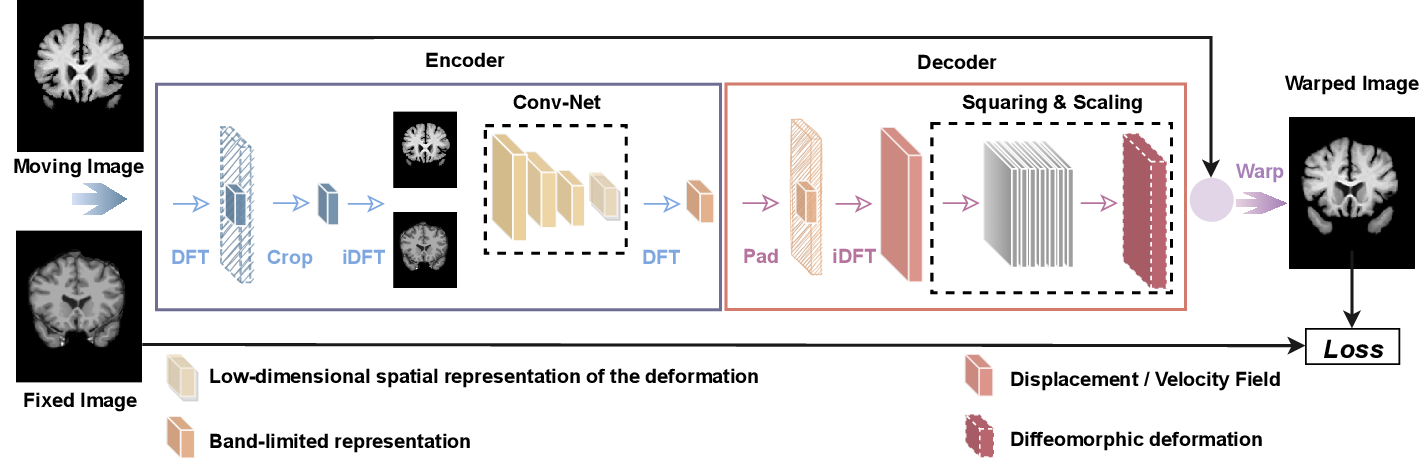
\includegraphics[width=\linewidth]{ArchitectureFourier-Net+.png} 
	\caption{Architecture of \emph{Fourier-Net+} taken from~\cite{Fourier-Net+}.}
	\label{fig:Fourier-Net+}
\end{figure}

\subsection{Changes to the Encoder}
What changes compared to \emph{Fourier-Net}?

\begin{figure}[htpb]
	\centering
	\graphicspath{{images/}{\main/images/}}
	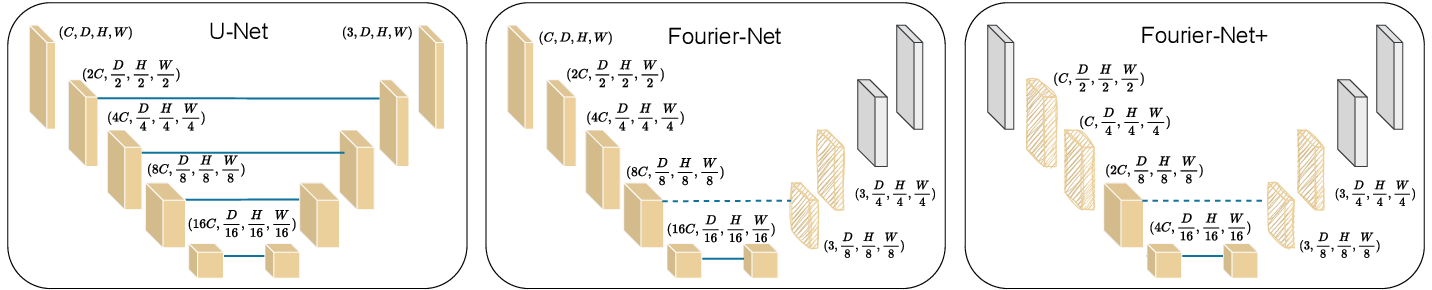
\includegraphics[width=\linewidth]{ArchitectureFourier-Net+CNN.png} 
	\caption{Architecture of the CNN for a typical U-Net, \emph{Fourier-Net} and \emph{Fourier-Net+} taken from~\cite{Fourier-Net+}.}
	\label{fig:Fourier-Net+CNN}
\end{figure}

\subsection{Effects of Cascading}
Why use cascaded version of the network?

\begin{figure}[htpb]
	\centering
	\graphicspath{{images/}{\main/images/}}
	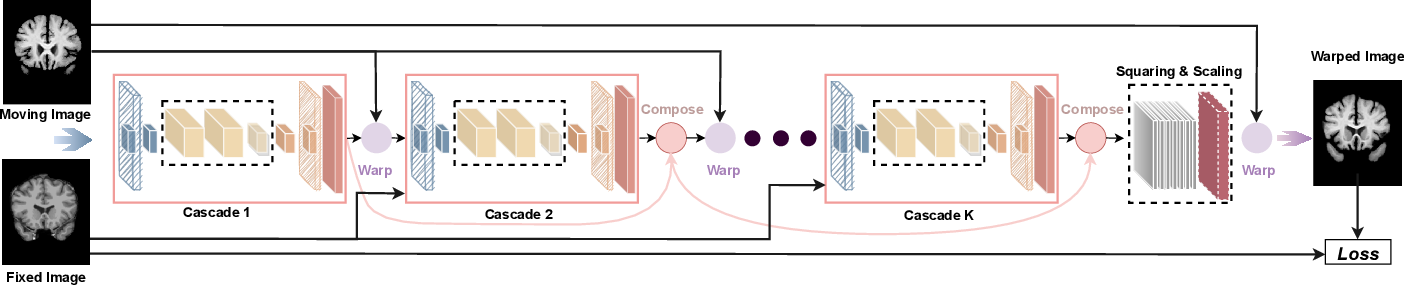
\includegraphics[width=\linewidth]{ArchitectureFourier-Net+Cascaded.png} 
	\caption{Cascaded version of \emph{Fourier-Net+} taken from~\cite{Fourier-Net+}.}
	\label{fig:Fourier-Net+Cascaded}
\end{figure}

\chapter{Experiments} %Evaluation
Describe the experiment and evaluation methods being used.
%Describe data here?!?


%%%%%%%%%%%%%%%%%%%%%%%%%%%%
%% Results and Discussion %%
%%%%%%%%%%%%%%%%%%%%%%%%%%%%

\chapter{Results and Discussion}
Here go the results with the discussion.


%%%%%%%%%%%%%%%%%%%%%%%
%%%%%  Conclusion %%%%%
%%%%%%%%%%%%%%%%%%%%%%%

\chapter{Conclusion}
Summery of all stuff...

\end{document}